\documentclass[11pt,a4paper]{article}

\usepackage[utf8]{inputenc}
\usepackage[T1]{fontenc}
\usepackage{amsmath,amssymb}
\usepackage{graphicx}
\usepackage{hyperref}
\usepackage{listings}
\usepackage{xcolor}
\usepackage{tikz}
\usetikzlibrary{shapes,arrows,positioning,fit,backgrounds}
\usepackage{algorithm}
\usepackage{algpseudocode}
\usepackage{booktabs}
\usepackage{geometry}
\geometry{margin=1in}

\title{Palace: Cascading LLM Control for Autonomous Software Development}
\author{Riff.CC}
\date{\today}

\definecolor{codegreen}{rgb}{0,0.6,0}
\definecolor{codegray}{rgb}{0.5,0.5,0.5}
\definecolor{codepurple}{rgb}{0.58,0,0.82}
\definecolor{backcolour}{rgb}{0.95,0.95,0.92}

\lstdefinestyle{mystyle}{
    backgroundcolor=\color{backcolour},
    commentstyle=\color{codegreen},
    keywordstyle=\color{magenta},
    numberstyle=\tiny\color{codegray},
    stringstyle=\color{codepurple},
    basicstyle=\ttfamily\footnotesize,
    breakatwhitespace=false,
    breaklines=true,
    captionpos=b,
    keepspaces=true,
    numbers=left,
    numbersep=5pt,
    showspaces=false,
    showstringspaces=false,
    showtabs=false,
    tabsize=2
}
\lstset{style=mystyle}

\begin{document}

\maketitle

\begin{abstract}
Palace is a development environment that enables autonomous AI agents to write,
test, and maintain software with human oversight.
We introduce \emph{cascading LLM control}, a technique where multiple language models
of varying capability operate in parallel, with a Director component dynamically
selecting which model makes decisions versus provides feedback based on task complexity
and cost constraints.
We also introduce \emph{transactional codegen}, a staged approach to code generation
where changes accumulate in shadow state and commit atomically only when validation
preconditions pass.
This paper describes the Palace architecture, its component interactions,
and presents preliminary results from deployment.
\end{abstract}

\section{Introduction}

Software development faces fundamental unsolved problems:
\begin{itemize}
    \item \textbf{The translation gap}: Human intent does not map cleanly to machine behavior.
    \item \textbf{The verification problem}: We discover if software works by watching it fail.
    \item \textbf{The maintenance trap}: Software accretes complexity until collapse.
    \item \textbf{The knowledge problem}: Context evaporates across developer boundaries.
\end{itemize}

Palace addresses these through:
\begin{itemize}
    \item Intent translation via LLM cascade
    \item Verification through Lean proofs and automated E2E testing
    \item Maintenance via recursive self-improvement
    \item Knowledge preservation through shared filesystem observation
\end{itemize}

\section{Architecture}

Palace consists of three layers: Human, Control, and Integration.

\subsection{Human Layer}

The human layer provides interfaces for human-AI collaboration:

\begin{itemize}
    \item \textbf{Conductor}: Resolves uncertainties through recursive interviews with
          branching questions. When the AI is uncertain, it asks rather than guesses.
    \item \textbf{Gamepad Input}: Full controller support for non-keyboard interaction.
    \item \textbf{Dual-Screen Rendering}: Program output alongside orchestration controls.
\end{itemize}

\subsection{Control Layer}

The control layer orchestrates AI decision-making:

\begin{itemize}
    \item \textbf{Director}: Autonomous project manager that creates issues,
          prioritizes work, and escalates to humans when needed.
    \item \textbf{Mountain}: Cascading LLM control with multiple model tiers.
    \item \textbf{llm-code-sdk}: Unified LLM API with code intelligence features.
\end{itemize}

\subsection{Integration Layer}

The integration layer connects to external systems:

\begin{itemize}
    \item \textbf{palace-plane}: Plane.so for project management
    \item \textbf{palace-gba}: GBA emulation for benchmark scenarios
    \item \textbf{palace-ci}: Dagger-powered CI pipelines
\end{itemize}

\begin{figure}[h]
\centering
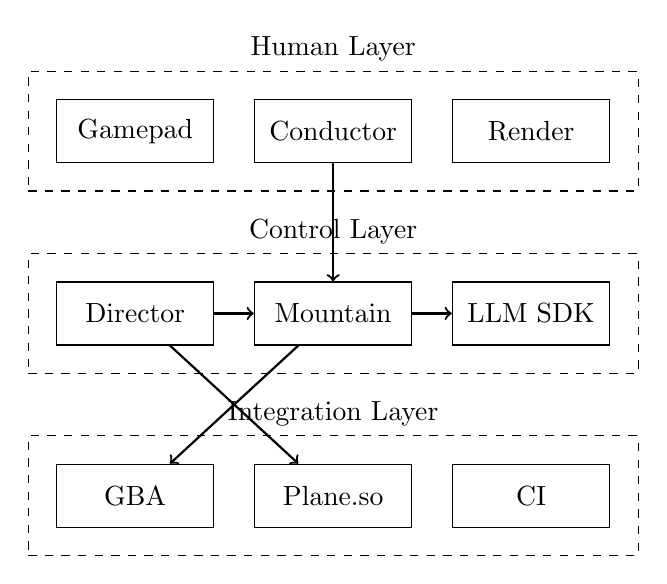
\begin{tikzpicture}[
    box/.style={rectangle, draw, minimum width=2cm, minimum height=0.8cm, align=center},
    layer/.style={rectangle, draw, dashed, inner sep=10pt},
    arrow/.style={->, thick}
]
    % Human Layer
    \node[box] (gamepad) {Gamepad};
    \node[box, right=0.5cm of gamepad] (conductor) {Conductor};
    \node[box, right=0.5cm of conductor] (render) {Render};

    % Control Layer
    \node[box, below=1.5cm of gamepad] (director) {Director};
    \node[box, right=0.5cm of director] (mountain) {Mountain};
    \node[box, right=0.5cm of mountain] (sdk) {LLM SDK};

    % Integration Layer
    \node[box, below=1.5cm of director] (gba) {GBA};
    \node[box, right=0.5cm of gba] (plane) {Plane.so};
    \node[box, right=0.5cm of plane] (ci) {CI};

    % Layer boxes
    \begin{scope}[on background layer]
        \node[layer, fit=(gamepad)(conductor)(render), label=above:Human Layer] {};
        \node[layer, fit=(director)(mountain)(sdk), label=above:Control Layer] {};
        \node[layer, fit=(gba)(plane)(ci), label=above:Integration Layer] {};
    \end{scope}

    % Arrows
    \draw[arrow] (conductor) -- (mountain);
    \draw[arrow] (director) -- (mountain);
    \draw[arrow] (mountain) -- (sdk);
    \draw[arrow] (director) -- (plane);
    \draw[arrow] (mountain) -- (gba);

\end{tikzpicture}
\caption{Palace architecture overview}
\label{fig:architecture}
\end{figure}

\section{Cascading LLM Control}

The core innovation in Palace is \emph{cascading LLM control},
implemented in the Mountain component.

\subsection{Model Tiers}

Palace operates multiple model tiers simultaneously:

\begin{table}[h]
\centering
\begin{tabular}{lll}
\toprule
\textbf{Tier} & \textbf{Model} & \textbf{Latency} \\
\midrule
FAST & nvidia\_orchestrator-8b & $\sim$200ms \\
FLASH & glm-4.7-flash & $\sim$500ms \\
MINI & ministral-3-14b-reasoning & $\sim$1s \\
FULL & glm-4.7 & $\sim$2s \\
OC & GPT-5.2, Opus, GPT-5.2-Pro & $\sim$3-5s \\
\bottomrule
\end{tabular}
\caption{Model tiers and typical latencies}
\label{tab:tiers}
\end{table}

\subsection{Assurance Levels}

The \emph{AssuranceLevel} determines which model makes decisions:

\begin{algorithm}
\caption{Cascade Decision Selection}
\begin{algorithmic}[1]
\State \textbf{Input:} AssuranceLevel $L$, Task complexity $C$
\State \textbf{Output:} Decision maker $D$, Feedback providers $F$
\If{$L = \text{FAST}$}
    \State $D \gets \text{8b}$
    \State $F \gets \{\text{flash}, \text{mini}, \text{full}\}$
\ElsIf{$L = \text{FULL}$}
    \State $D \gets \text{glm-4.7}$
    \State $F \gets \emptyset$
\ElsIf{$L = \text{FULL+OC}$}
    \State $D \gets \text{glm-4.7}$
    \State $F \gets \{\text{GPT-5.2}, \text{Opus}, \text{GPT-5.2-Pro}\}$
\EndIf
\State \textbf{return} $D$, $F$
\end{algorithmic}
\end{algorithm}

\subsection{Director Autonomy}

The Director autonomously adjusts the AssuranceLevel based on:
\begin{itemize}
    \item Task complexity (simple rename vs architectural change)
    \item Cost constraints (local models vs cloud API costs)
    \item Risk level (reversible change vs breaking change)
    \item Historical accuracy (model performance on similar tasks)
\end{itemize}

\section{Transactional Codegen}

Traditional code generation writes changes immediately.
Palace introduces \emph{transactional codegen}, where changes accumulate
in shadow state and commit atomically.

\subsection{Transaction Stages}

\begin{enumerate}
    \item \textbf{Setup}: Define preconditions (compilation, tests, custom checks)
    \item \textbf{Build}: Accumulate shadow edits across files
    \item \textbf{Validate}: Check preconditions in isolated environment
    \item \textbf{Commit}: Apply atomically when all preconditions pass
\end{enumerate}

\subsection{Git Worktree Integration}

Validation runs in git worktrees for proper isolation:

\begin{lstlisting}[language=bash]
git worktree add ../shadow-<tx> -b shadow/<tx>
# Apply shadow edits
# Run validation (compile, test)
git worktree remove ../shadow-<tx>
\end{lstlisting}

\subsection{Benefits}

\begin{itemize}
    \item \textbf{Arbitrarily large changesets}: Entire codebase refactors become tractable
    \item \textbf{Validation gates}: Changes only apply when proven correct
    \item \textbf{Iterative refinement}: Model can retry until validation passes
    \item \textbf{Atomic commits}: No partial states in the repository
\end{itemize}

\section{Branch Strategy}

Palace employs a three-tier branch strategy:

\begin{table}[h]
\centering
\begin{tabular}{lll}
\toprule
\textbf{Branch} & \textbf{Purpose} & \textbf{CI Tier} \\
\midrule
main & Production releases & Release ($\sim$hours) \\
dev & Rolling release & Dev ($\sim$10min) \\
feature & Work in progress & Draft ($<$5s) \\
\bottomrule
\end{tabular}
\caption{Branch strategy}
\label{tab:branches}
\end{table}

Changes graduate between branches using the same transactional codegen process,
ensuring each tier's validation requirements are met.

\section{Preliminary Results}

\textit{This section will be updated with deployment data as Palace matures.}

\subsection{Metrics to Track}

\begin{itemize}
    \item Task completion rate by AssuranceLevel
    \item Validation pass rate on first attempt
    \item Cost per successfully merged change
    \item Time from intent to merged code
    \item Human intervention frequency
\end{itemize}

\section{Related Work}

Palace builds on ideas from:
\begin{itemize}
    \item Agentic coding assistants (Claude Code, Cursor, Aider)
    \item Model cascading and routing (Anthropic's model selection)
    \item Formal verification (Lean, Coq)
    \item Transactional systems (database ACID properties)
\end{itemize}

\section{Future Work}

\begin{itemize}
    \item Lean proof integration for verified code generation
    \item Multi-agent coordination via Zulip channels
    \item Continuous background improvement when idle
    \item Cross-repository refactoring transactions
\end{itemize}

\section{Conclusion}

Palace demonstrates that cascading LLM control and transactional codegen
can make autonomous software development tractable.
By dynamically selecting decision makers based on complexity and cost,
and by validating changes before committing,
Palace achieves reliable code generation at scale.

\bibliographystyle{plain}
% \bibliography{references}

\end{document}
